\documentclass{article}
\usepackage{arxiv}
\usepackage[T1]{fontenc}
\usepackage{microtype}
\usepackage{amsmath,amssymb,graphicx,booktabs}
\usepackage[round,authoryear]{natbib}
\usepackage[hidelinks]{hyperref}
\setlength{\emergencystretch}{3em}
\setlength{\tabcolsep}{3pt}
\title{Opal: single-informed prediction of expression and combinatorial growth}
\author{Arjun Vijay Prakash\\The Tiny Intelligence Lab\\Independent researcher}
\date{}
\renewcommand{\shorttitle}{Opal: expression and combinatorial growth}
\renewcommand{\undertitle}{Opal v1.0.0 research release}
\hypersetup{pdftitle={Opal: single-informed prediction of expression and combinatorial growth},pdfauthor={Arjun Vijay Prakash},pdfsubject={Computational perturbation biology},pdfkeywords={combinatorial perturbations, residual kernels, generalization, reproducibility}}
\newcommand{\NormanGain}{15.81}
\newcommand{\WesselsGain}{61.08}
\newcommand{\DspinCandidate}{0.034025}
\newcommand{\DspinReference}{0.033108}

\begin{document}
\maketitle

\begin{abstract}
Measured single perturbations constrain combination responses but do not identify arbitrary interactions. Opal evaluates symmetric residual models for population-mean expression and double-CRISPRi growth with matched simple references. Historical expression networks improve over additivity, but their advantage over selected simple references is inconclusive or negative; a later expression-composition hypothesis also fails. An original growth experiment improves held-pair MSE by 26.44\% in K562 and 14.82\% in Jurkat relative to calibrated main effects, while joint context sharing fails promotion. Frozen K562 transfer then fails on four external cohorts, with 1.08--2.15\% higher MSE than frozen main effects. A later source-local benchmark pools five disjoint test blocks in six already exposed growth tasks. Completion reduces MSE relative to selected simple references by 5.80\%, 4.11\%, 25.14\%, 28.75\%, 17.56\% and 13.95\% for K562, Jurkat, two environmental cohorts and two PARPi cohorts, respectively. Jurkat misses the registered 5\% threshold, so the all-task promotion criterion fails. These local results require measured singles and substantial pair supervision among supported genes; they do not reverse unsuccessful frozen transfer. Negative low-label, state/context, composition and numerical-compatibility findings remain part of the evidence. Opal v1 provides inspectable code, protocols and aggregate results, with trained models reserved for separate distribution. No biological discovery, causal interaction identification, calibrated biological uncertainty or frontier-level superiority is established.
\end{abstract}
\noindent\textbf{Keywords:} combinatorial perturbations; expression; CRISPRi growth; matrix completion; source transfer; reproducibility; evaluation.

\section{Introduction}
Single-cell perturbation experiments connect interventions to transcriptional responses, while combinatorial screens measure departures from single-intervention behavior. Norman's K562 CRISPR activation experiment provides a widely used genetic combination dataset \citep{norman2019}. CaRPool-seq extends combinatorial targeting to RNA transcripts using Cas13 and provides a second experimental system \citep{wessels2023}. These experiments motivate a prediction task that is narrower than general perturbation prediction: given measured single profiles in one context, predict an unmeasured simultaneous pair.

The additive prediction supplies a strong starting point. A learned model can improve on it by capturing a shared calibration error, a common offset, or pair-specific structure. Only the last explanation supports a claim that particular pair features contribute useful information. Metric calibration also matters because errors across many weakly responding genes and correlations dominated by single effects can obscure the quality of interaction prediction \citep{ahlmann2025,miller2026}. We therefore compare the proposed correction to stronger controls using the same observed singles, and assess synthetic negative controls before interpreting biological gains.

This work implements Opal as a family of single-informed residual models and an auditable experimental pipeline. The present contribution is the controlled internal comparison and its negative predictive findings on the observed datasets. No state-of-the-art or independent biological validation claim follows. Residual subtraction, symmetry, and dimensionality restriction are established modeling tools. The experiments ask which of these restrictions help under a frozen selection procedure, and retain unfavorable results. The historical expression scope is preserved. The present update adds a distinct functional growth endpoint, a locked external-screen test and explicitly exploratory failure diagnostics. Growth accuracy does not establish transcriptomic accuracy, and repeated computational development does not create untouched confirmation.

A dense growth screen provides a complementary test of the information bottleneck: can measured singles plus many observed combinations support missing-pair prediction, and does that signal survive a different screen? The answer separates a within-source completion gain from a failed unchanged-model external claim. Post-failure diagnostics distinguish reproducible pair alignment, assay-local main effects and graph support without replacing the original result.

\begin{figure}[htbp]\centering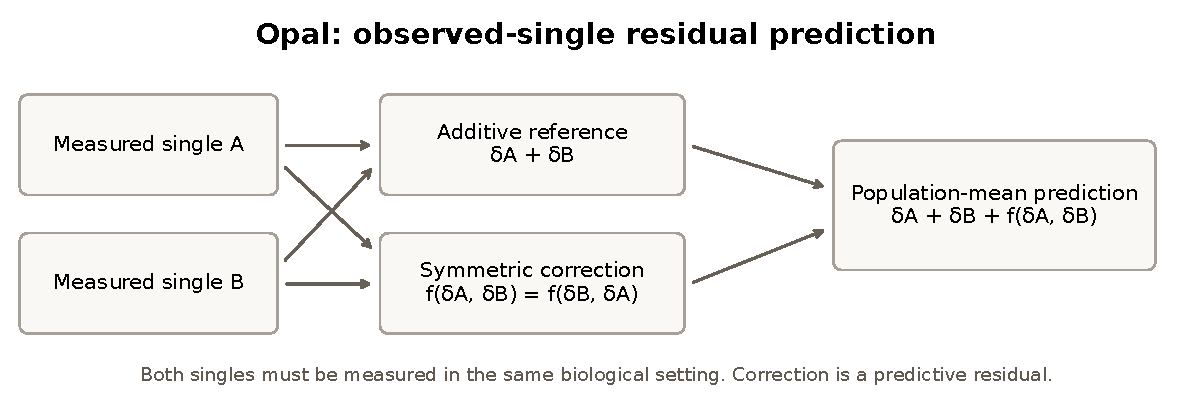
\includegraphics[width=\linewidth]{evidence/opal_overview.pdf}\caption{The observed-single prediction contract. A symmetric correction is added to two measured effects; its residual target includes shared distortion and measurement error as well as possible pair-specific structure.}\label{fig:overview}\end{figure}

\section{Related work}
CPA learns compositional representations for predicting responses to complex perturbations and supplies the earlier chemical feasibility source considered here \citep{cpa2023}. GEARS uses biological knowledge graphs to predict multigene perturbation responses \citep{gears2024}. Neither a published score under a different split nor access to external knowledge is interchangeable with a comparison that supplies observed singles under our protocol. Our internal controls use the same inputs. Later native CPA and GEARS aggregate adaptations are reported separately below, with their departures from canonical cell-level evaluation disclosed.

NAIAD combines single-effect information and learned representations for combinatorial experimental discovery \citep{naiad2025}. Its phenotype and acquisition objectives constrain claims of novelty for any single-informed pair model, but a transcriptomic comparison requires compatible outputs and data access. SLIM supplies a small linear reference using STRING embeddings \citep{slim2026}; its upstream resource must be accounted for separately. PertAdapt adapts single-cell foundation models to perturbation prediction \citep{pertadapt2026}, so upstream pretraining and combination-task compatibility must also be disclosed. These references motivate future controlled benchmarks; no result in this manuscript ranks Opal against these methods.

\section{Methods}
\subsection{Task and expression scale}
Let $\mu_{u,s,g}$ denote the mean library-normalized count for intervention $u$, matched stratum $s$, and gene $g$, and let $\mu_{0,s,g}$ denote its control mean. Each cell is normalized to the median retained control library total. The primary effect is
\begin{equation}
\delta_{u,g}=\frac{1}{|S_u|}\sum_{s\in S_u}\left[\log_2(1+\mu_{u,s,g})-\log_2(1+\mu_{0,s,g})\right].
\end{equation}
We transform condition means, rather than averaging transformed cell counts. Strata contribute equally, and a retained pair must share stratum support with both component singles. The source-specific stratum definitions are technical matching variables, not assumed independent biological replicates.

For two distinct simultaneous interventions $A$ and $B$, define $a_{AB}=\delta_A+\delta_B$ and $r_{AB}=\delta_{AB}-a_{AB}$. The prediction is
\begin{equation}\widehat\delta_{AB}=a_{AB}+f_\theta(\delta_A,\delta_B),\qquad f_\theta(\delta_A,\delta_B)=f_\theta(\delta_B,\delta_A).\label{eq:model}\end{equation}
In the historical genetic benchmark, all components have observed single profiles in the same experimental context. That protocol does not evaluate unseen singles, different cell types, different doses, sequential treatments, or individual-cell trajectories. Additivity depends on the chosen expression scale, and $r_{AB}$ also includes error in the estimated singles and controls. It is a prediction residual, not automatically drug synergy or a causal genetic mechanism.

Residual and response losses are identical when the observed additive term is fixed:
\begin{equation}\|f_\theta-r_{AB}\|_2^2=\|a_{AB}+f_\theta-\delta_{AB}\|_2^2.\end{equation}
Any benefit from residual training therefore arises from parameterization, initialization, or regularization, rather than a different squared-error objective.

\subsection{Source preparation and input access}
Norman uses the named secondary scPerturb release from Zenodo record 7278143 version 1.1 \citep{scperturb2024state}. Its documented transformation reads the original count matrix without expression normalization. We retain source-annotated good-coverage singlet assignments and explicitly negative-control constructs, preserve guide provenance, and match by gemgroup. This is distinct from a GEARS compatibility track. The initial library range is 500--20,000 counts, with at least 50 cells per condition. After source-specific exclusions and target-pair aggregation, the prepared dataset has 105 singles, 126 pairs, and 10,623 eligible genes; 88 pairs are development conditions and 38 are final test conditions.

Wessels uses the original GSE213957 four-lane archive and THP1 metadata \citep{wessels2023}. Barcode joins retain metadata-matched THP1 Gene Expression measurements and exclude HEK293 cells and guide-count features. Exact \texttt{NT} tokens determine controls, avoiding substring misclassification of target names. The minimum library is 500; the maximum is the 99.5th percentile of controls and singles. Conditions require at least 50 cells, and lanes supply matched strata. Many measured singles fail this minimum, so the accepted task covers 16 singles and 58 pairs, with 10,590 genes, 40 development pairs, and 18 test pairs. This restricted coverage is a consequence of the observed-single contract.

Gene eligibility uses controls and singles only. A gene survives if at least one reference condition has normalized mean at least 0.1 and detection fraction at least 0.01. This frozen universe is the primary output; it does not establish performance on genes excluded by the reference rule. Source hashes, count locations, guide mapping, exclusions, normalization parameters, gene order, and split manifests are retained. Held-out pair responses occupy a separate evaluator bundle and are unavailable to model fitting or architecture selection.

\IfFileExists{evidence/coverage.pdf}{\begin{figure}[ht]\centering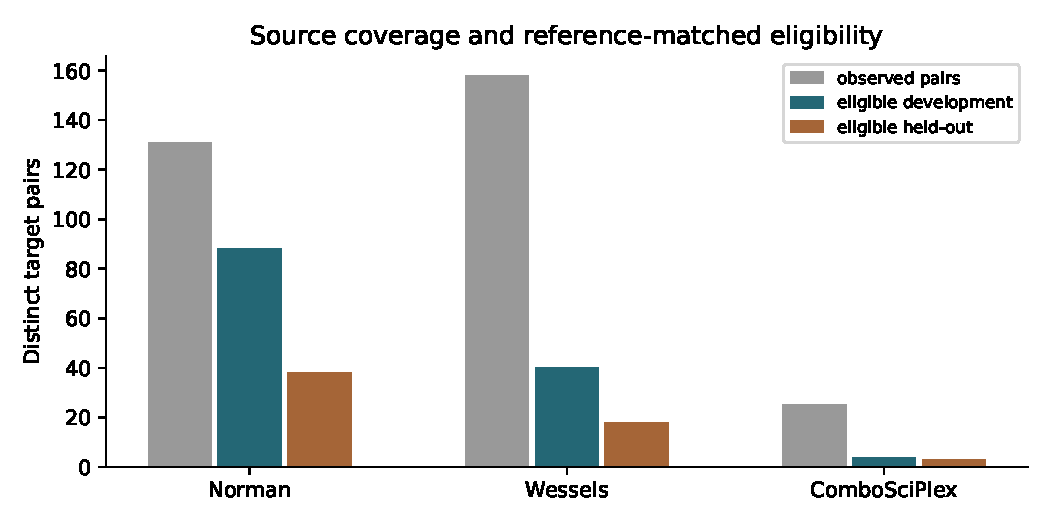
\includegraphics[width=0.85\linewidth]{evidence/coverage.pdf}\caption{Original distinct nonrepeat pair coverage and surviving reference-matched development/test conditions. Source-level measurement does not guarantee a usable pair with both matched singles.}\end{figure}}{}

\subsection{Representations and correction families}
PCA fitted to centered single effects supplies an embedding $e_u\in\mathbb R^m$. Its dimension is capped by the number of available singles and output genes; nominal dimensions are 32 for Norman and 16 for Wessels and the synthetic suite. An identity representation and a linear denoising encoder are comparison candidates. When split-half single profiles exist, the encoder learns reciprocal reconstruction between halves. Otherwise, the synthetic comparison uses added noise. Joint fine-tuning updates the target embedding table with a single-profile reconstruction penalty; it is not a demonstrated encoder for previously unmeasured targets.

The coordinate-product model uses $q_{AB}=e_A\odot e_B$. A learned bilinear candidate uses
\begin{equation}q_{AB}=(Pe_A)\odot(Pe_B),\qquad f_\theta=b+B\Lambda^\top q_{AB},\end{equation}
where $B\in\mathbb R^{G\times k}$ defines a shared output space. An independent symmetric-form candidate uses coordinates $e_A^\top W_j e_B$ with symmetric $W_j$. The neural network candidate applies a tanh network to concatenated $e_A+e_B$, $|e_A-e_B|$, and projected products. Its sum-network control omits the projected-product block but retains the sum and absolute difference. We therefore call this control a network without multiplicative features, rather than claiming that it receives only the sum. Both networks predict coefficients in the output basis plus an optional offset. Unrestricted-output, fixed-basis, zero-offset, random-initialization, direct-response, representation, and fine-tuning comparisons test individual choices.

\subsection{Baselines and development selection}
The internal baseline set includes no-change, additive, training-mean response, training-mean residual, symmetric ridge regression, reduced-rank regression, nearest-neighbor residual correction, and global correction. Symmetric regression uses sum, absolute difference, and coordinate products of the same embeddings. Global correction uses the observed additive response directly, with an optional feature expansion comprising its coordinates, their hyperbolic tangents, and their squares. It can explain shared nonlinear distortions without using pair identities.

Random pair holdout reserves 30\% of canonical unordered pairs, using identities alone. Five development folds determine candidate errors and stopping epochs. The initial CPU search uses ranks 2 and 8, ridge penalties 1 and 100, and at most 80 epochs for neural candidates. AdamW uses learning rate 0.01 and weight decay 0.01, with full-batch equal-condition loss. Initial screening uses one optimization seed; real-data finalist evaluation uses five seeds, while synthetic engineering finalists use two. Final neural predictions average five refitted seeds. The selected neural family and the selected simpler comparator are chosen separately on development error and fixed before final evaluation. Their comparison can therefore reject the neural structural claim even when the network beats additivity.

Within each development fold, the validation responses choose the best neural stopping epoch and score that checkpoint. Candidate scores average member-specific errors across seeds, rather than scoring a seed-averaged ensemble. Final refits use the median selected epoch across folds and seeds, then average predictions from five seeds before scoring. Development errors are model-selection scores, not unbiased estimates of final ensemble error. For partner cross-validation, predictions from overlapping validation folds are averaged per covered pair before computing each seed's score; uncovered pairs do not contribute.

This bounded search is the initial registered implementation batch, not the an exhaustive capacity comparison. Learning curves use nested development subsets and three subset orders while keeping the full-development-selected hyperparameters. They measure fixed-hyperparameter sensitivity, rather than a subset-retuned sample-efficiency optimum. Additional combination-partner holdouts remove all development pairs incident to specified held targets while preserving their single profiles. Partner folds may overlap in their test pairs and cannot be counted as independent experiments.

\subsection{Classical residual kernels}
The exploratory genetic kernel family operates directly on observed single-effect profiles. For reference singles $x_u=\delta_u$, the radial kernel is $k_{uv}=\exp[-\lVert x_u-x_v\rVert_2^2/(h d_0)]$, where $d_0$ is the median positive pairwise squared distance between permitted reference singles and $h>0$ is a selected bandwidth. Two symmetric pair kernels are
\begin{align}
K_{\Sigma}(AB,CD)&=(k_{AC}+k_{AD}+k_{BC}+k_{BD})/4,\\
K_{\Pi}(AB,CD)&=(k_{AC}k_{BD}+k_{AD}k_{BC})/2.
\end{align}
The global kernel is the linear Gram matrix of the scaled additive response, divided by the gene count; its per-gene scale is $\max(\sqrt{2}\,\operatorname{sd}(x_{u,g}),10^{-6})$. Candidates include a shared offset, global correction, the sum kernel, the pair-product kernel, and global-plus-pair mixtures with registered unit or tenfold pair weights. Neither a pair-product form nor a favorable total error is alone evidence of biological interaction learning.

For $n$ training pairs, $H=I-\mathbf{1}\mathbf{1}^{\mathsf T}/n$ centers the training Gram matrix $K$. With residual matrix $R$ and mean $\bar r$, the fitted coefficients are
\begin{equation}C=(HKH+\alpha I)^{-1}(R-\mathbf{1}\bar r^{\mathsf T}),\qquad \widehat r(q)=\bar r+k_c(q)C.\end{equation}
Here $k_c(q)$ uses training kernel means for query centering. The mean residual is an unpenalized intercept; $\alpha>0$ is selected using development folds. This is closed-form regularized regression, with stored references and coefficients counted in its resource cost.

The contextual amendment uses a separate implementation. It standardizes genes using all explicitly permitted measured single references, including query-context singles, and estimates the reference-distance scale from at most 512 seed-fixed reference profiles. Component kernels are normalized by training diagonal means. Context-conditioned candidates multiply the pair kernel by an RBF of control-derived context features, standardized using source training contexts. A weighted global component and a pooled pair component are optional. These reference allowances make this transductive observed-reference transfer, rather than zero-shot prediction from an unseen context without measured singles. No held-context pair outcome sets reference normalization or fits the source response coefficients.

\subsection{Endpoints and uncertainty}
For $N$ test pairs and $G$ frozen genes, the primary endpoint and additive skill are
\begin{equation}\operatorname{MSE}=\frac{1}{NG}\sum_{p,g}(\widehat\delta_{p,g}-\delta_{p,g})^2,\qquad \operatorname{skill}_{\rm add}=1-\frac{\operatorname{MSE}_{\rm model}}{\operatorname{MSE}_{\rm additive}}.\end{equation}
Pairs have equal weight regardless of cell count. Secondary artifacts record absolute error, response correlation, residual alignment, component-informed panel error, and residual geometry. Component panels use single effects and control dispersion where available, without examining held-out doubles. Evaluator-only emergent-response analyses do not define the fitting gene universe.

Paired improvement is baseline MSE minus selected-model MSE. We report 2,000-draw pair bootstrap and target-product-weight bootstrap sensitivities. These are descriptive intervals conditional on estimated profiles and the fitted selection. They do not propagate shared-control uncertainty, the full measurement process, model selection, or independent biological replication. Split-half profiles provide a measurement-reliability diagnostic, not an accuracy ceiling. Ensemble dispersion is not a calibrated confidence interval or a validated abstention policy.

\subsection{Synthetic engineering suite}
The suite uses 24 targets, 96 genes, and all 276 unordered distinct pairs. Eight generators produce log-scale additivity, count-scale additivity evaluated on a log scale, low-rank interactions, cross-coordinate interactions, higher-rank interactions, a shared nonlinear additive-response distortion, emergent effects in genes without single effects, and noisy singles with a shared control error. Pair responses receive Gaussian observation noise with standard deviation 0.015. Five total random splits and five partner folds are completed for the low-rank generator. These constructed tasks validate implementation behavior and identifiable failure modes; they do not establish biological performance or prevalence of low-rank interactions.

\section{Results}
\subsection{Synthetic recovery depends on the generating structure}
\IfFileExists{evidence/table.tex}{\begin{table}[ht]\centering\normalsize\begin{tabular}{llrrr}
\toprule
Scenario & Selected family & MSE & Skill & Simpler MSE \\
\midrule
additive log & bilinear & 0.00022 & -0.000 & 0.00022 \\
additive count & bilinear & 0.00050 & 0.471 & 0.00054 \\
low rank & network & 0.00035 & 0.968 & 0.00598 \\
cross coordinate & network & 0.00026 & 0.956 & 0.00240 \\
high rank & bilinear & 0.00943 & 0.657 & 0.01134 \\
global distortion & network & 0.00110 & 0.941 & 0.00104 \\
emergent & network & 0.00024 & 0.859 & 0.00085 \\
noisy controls & network & 0.00241 & 0.842 & 0.00562 \\
\bottomrule
\end{tabular}
\caption{Completed synthetic suite. Scores are equal-pair held-out mean squared errors and additive skill as a fraction. These are engineering tasks, not biological validation.}\label{tab:synthetic}\end{table}}{}
The log-additive negative control has selected MSE $2.22709\times10^{-4}$ and additive skill $-0.019\%$, so residual learning supplies no useful gain. The low-rank and cross-coordinate generators yield skills of 96.76\% and 95.63\%, respectively, for development-selected symmetric networks. Their selected errors are $3.48993\times10^{-4}$ and $2.57490\times10^{-4}$. This demonstrates recovery when the synthetic structure is learnable under the implemented information access.

\IfFileExists{evidence/synthetic_skill.pdf}{\begin{figure}[ht]\centering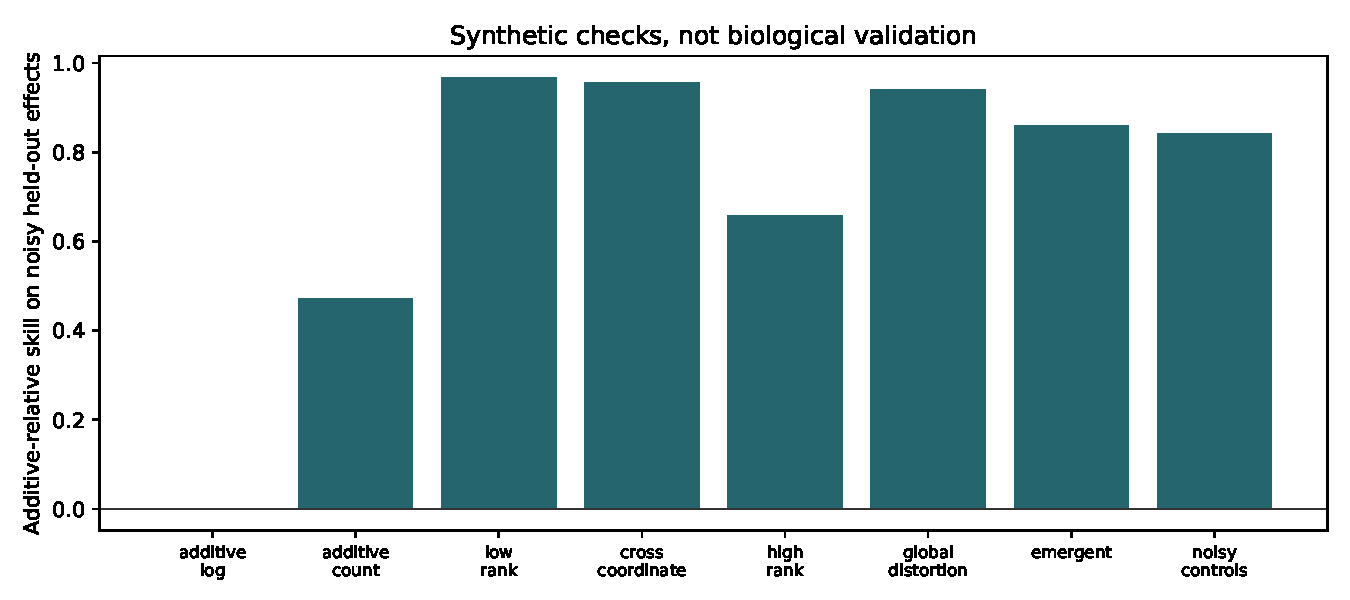
\includegraphics[width=0.96\linewidth]{evidence/synthetic_skill.pdf}\caption{Additive skill across synthetic mechanisms. Positive skill measures predictive improvement, not mechanistic evidence. The shared-distortion case requires comparison to the global correction.}\end{figure}}{}
The count-additive generator produces 47.10\% skill on the log endpoint, although its underlying count-scale generator has no added interaction. This illustrates scale dependence. In the global-distortion scenario, selected neural skill is 94.13\%, but its MSE $0.00110447$ exceeds the simpler correction's $0.00104015$. A large gain over additivity can therefore coexist with failure of the pair-model claim. The higher-rank scenario selects an unrestricted-output bilinear candidate and yields 65.71\% skill; this result does not support a universal low-rank restriction. Emergent and noisy-control scenarios produce 85.95\% and 84.24\% skill within their constructed universes.

Across the five random splits of the low-rank generator, selected skill ranges from 96.58\% to 97.42\%. Five partner folds yield 92.97\%--96.63\% skill, with 86 or 105 test pairs per fold. Generalization survives this harder synthetic split, but variation across held target groups and overlap among test sets limit interpretation. These results cannot substitute for real-data partner holdouts.

\subsection{Norman improves over additivity without a clear structural advantage}
\IfFileExists{evidence/biological_table.tex}{\begin{table}[ht]\centering\begin{tabular}{llrrrr}
\toprule
Dataset/scale & Neural family & Additive MSE & Neural MSE & Simpler MSE & Skill \\
\midrule
Norman (log) & network & 0.00852 & 0.00717 & 0.00727 & 0.158 \\
Wessels (log) & sum network & 0.01394 & 0.00542 & 0.00421 & 0.611 \\
Norman (count) & sum network & 1.24605 & 1.03911 & 1.25944 & 0.166 \\
Wessels (count) & sum network & 0.26123 & 0.19684 & 0.16913 & 0.246 \\
Chemical (exploratory) & bilinear & 0.01381 & 0.01223 & 0.00994 & 0.114 \\
\bottomrule
\end{tabular}
\caption{Completed primary biological results and available count sensitivity. Architecture and comparator selection use development data only. Skill is a fraction, and errors across expression scales are not directly comparable.}\label{tab:biological}\end{table}}{}
On 38 withheld Norman pairs, the selected rank-two symmetric network has MSE $0.007169187$, compared with $0.008515040$ for additivity, giving 15.81\% skill. Its separately development-selected reduced-rank regression comparator has MSE $0.007268184$. The selected network's paired improvement is only $0.0000989974$, with descriptive pair-bootstrap interval $[-0.000239746,0.000393522]$ and target-product-weight interval $[-0.000477775,0.000691408]$. Both cross zero, so the structural comparison is inconclusive under these conditional summaries.

An ordinary ridge candidate has the lowest observed classical test MSE, $0.006891604$, and 19.07\% additive skill. This candidate was not the frozen development-selected simpler comparator. Its favorable test score is a descriptive comparison among prespecified evaluated candidates, not grounds to select a replacement after viewing the test. It nevertheless prevents a broad claim that the selected network outperforms the evaluated classical alternatives.

\IfFileExists{evidence/norman-log2-primary-baselines.pdf}{\begin{figure}[ht]\centering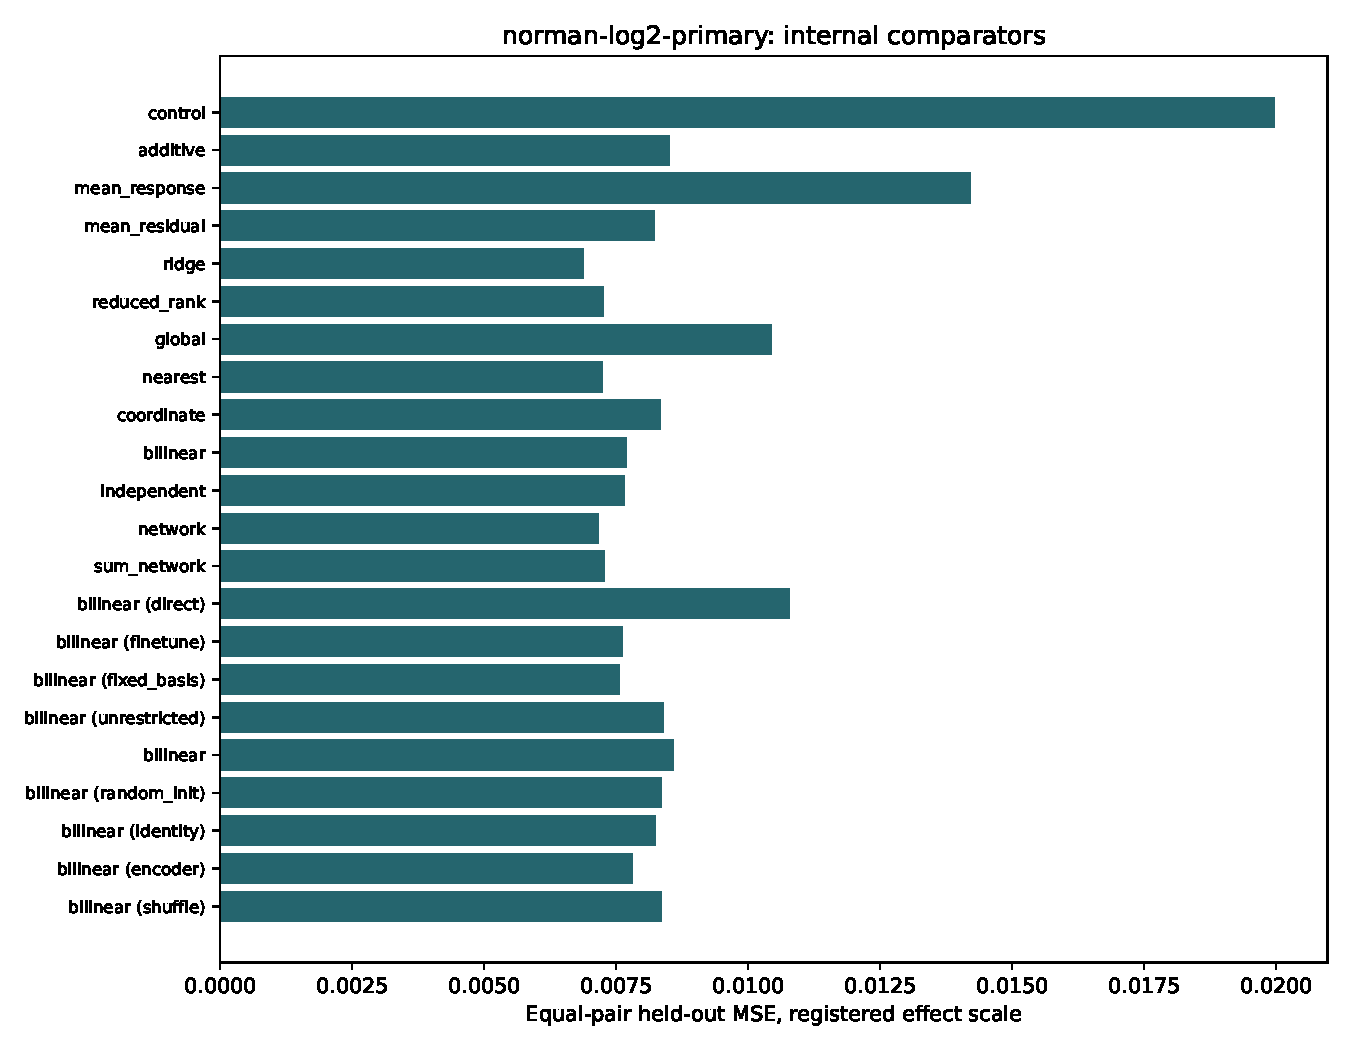
\includegraphics[width=0.95\linewidth]{evidence/norman-log2-primary-baselines.pdf}\caption{Norman primary internal comparisons. The development-selected neural model and simpler comparator are fixed before test access; the best observed test candidate does not become a new selection.}\end{figure}}{}

\subsection{Wessels improvement is explained more effectively by a global correction}
On 18 withheld Wessels pairs, the selected rank-eight network without multiplicative features has MSE $0.005423558$, compared with $0.013936912$ for additivity. Its additive skill is 61.08\%. The separately development-selected global correction has MSE $0.004214949$ and skill 69.76\%, so the selected network is worse by $0.001208610$ MSE. Pair-specific multiplicative structure has not demonstrated an advantage in this primary experiment.

For the network-minus-global comparison expressed as improvement, the descriptive pair-bootstrap interval is $[-0.00155317,-0.00091829]$, and the target-product-weight interval is $[-0.00189104,-0.00070451]$. Both favor the global correction conditional on these estimated profiles. They are not confirmatory population intervals. The additive comparison is positive under both descriptive schemes, but it cannot distinguish a general correction from pair-specific interaction learning. The selected model's omission of multiplicative features further limits the original architectural hypothesis.

The Wessels count-scale sensitivity also selects the network without multiplicative features. Its MSE is $0.19684419$, versus $0.26122700$ for additivity and $0.16912624$ for the development-selected simpler comparator. Skills are 24.65\% and 35.26\%, respectively. The negative neural-versus-simpler conclusion persists on this alternative scale, although the magnitudes of count and log errors are not comparable.

Norman count-scale sensitivity selects a rank-eight network without multiplicative features, with MSE $1.03911249$ versus additive $1.24604893$, giving 16.61\% skill. Its development-selected ridge comparator has MSE $1.25943739$. The neural improvement over ridge is $0.22032490$, but the descriptive pair interval $[-0.06229010,0.53790781]$ and target-product-weight interval $[-0.26011966,0.85000429]$ both cross zero. The count-scale target-weight interval for improvement over additivity also crosses zero. Scale sensitivity therefore supports neither a stable product-feature selection nor a resolved classical-versus-neural advantage.

\IfFileExists{evidence/wessels-log2-primary-baselines.pdf}{\begin{figure}[ht]\centering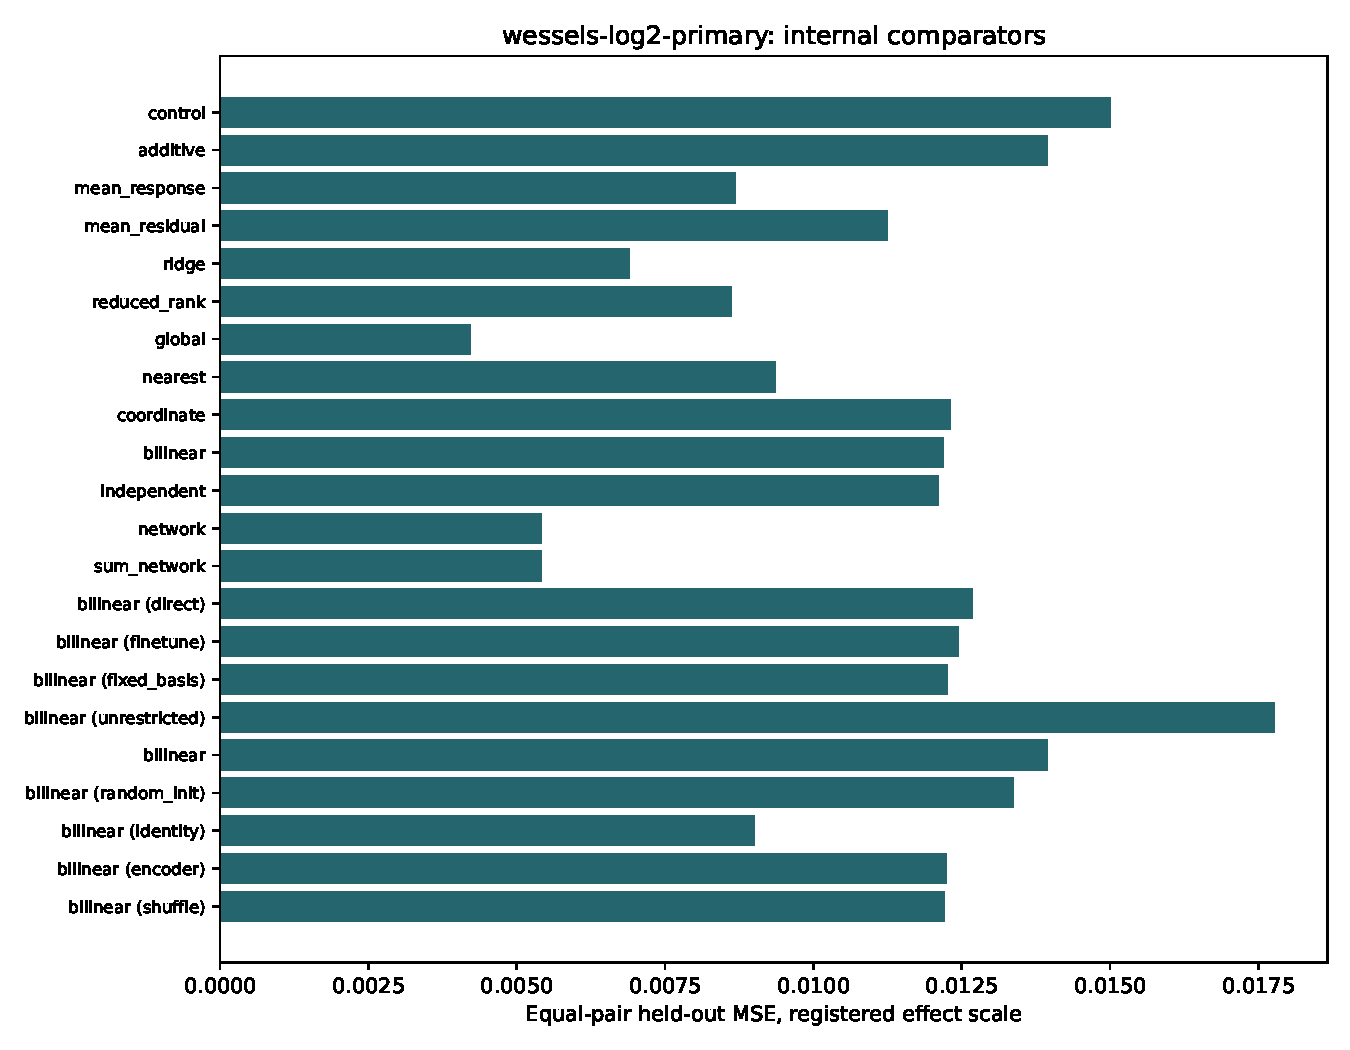
\includegraphics[width=0.95\linewidth]{evidence/wessels-log2-primary-baselines.pdf}\caption{Wessels primary internal comparisons. The global correction outperforms the selected network under the same observed-single input contract.}\end{figure}}{}

\subsection{Reliability and computational diagnostics}
Mean split-half residual cosine is 0.2891 for Norman and 0.0838 for Wessels. These technical partitions indicate substantial instability in the estimated interaction residuals; they are neither independent biological replicates nor an upper bound on prediction accuracy. An evaluator-only, swapped-half emergent panel of 20 genes per pair gives MSE 0.2401 and 0.1268, respectively. This diagnostic covers only the primary frozen gene universe, so it cannot establish recovery of genes excluded during reference-based filtering.

Ensemble-spread versus pair-error Pearson correlations are 0.5262 and 0.5835 on development out-of-fold predictions for Norman and Wessels, and 0.5441 and 0.3124 on their tests. These associations do not calibrate a failure probability, and no risk threshold is selected. Retrieval against the run's held-out responses identifies 35 of 38 Norman pairs and 17 of 18 Wessels pairs, compared with chance rates $1/38$ and $1/18$. Retrieval is sensitive to candidate composition and signal strength, so it supplements expression-error evaluation rather than replacing it. Prespecified best, median, and worst error examples are retained without selecting appealing biological narratives.

Selected five-member ensemble checkpoints occupy 6,079,406 bytes for Norman and 5,439,360 bytes for Wessels. With one CPU thread and 100 warm measurements, median single-pair prediction takes 0.676 and 0.751 milliseconds; 95th percentiles are 0.797 and 1.015 milliseconds. Cold checkpoint load takes 47.0 and 45.7 milliseconds. These retained measurements are saved separately as immutable timing records. They describe this machine and artifact layout, not an end-to-end request service. A separate fresh-process measurement after loading and 100 predictions reports peak resident working sets of 222,375,936 and 223,993,856 bytes, including Python and native-library overhead. Training peak memory was not measured. Baseline, capacity, fixed-hyperparameter learning-curve, residual-geometry, reliability, and example figures are generated alongside the result artifacts.

\subsection{Repeated random and combination-partner holdouts}
The biological secondary suite completes four additional random-pair seeds per dataset, giving five random splits including the primary, plus five combination-partner holdouts per dataset. Every split independently repeats development selection and final refitting under the same bounded protocol. Partner holdouts exclude development doubles incident to their held targets but retain those targets' measured singles; inner validation uses analogous partner splits. Gene eligibility and normalization remain fixed from allowed references. Overlapping test pairs and shared profiles make these sensitivity runs correlated, rather than independent experimental replications.

Norman neural additive skill ranges from 0.0820 to 0.1581 across random splits and from 0.0111 to 0.1607 across partner splits. Improvement over the independently development-selected simpler method is positive in one of five random splits and four of five partner splits, with partner differences spanning $-0.0000812$ to $0.0017721$ MSE. This protocol dependence does not establish a general structural advantage. Wessels additive skill ranges from 0.5067 to 0.6161 across random splits and 0.2106 to 0.3220 across partner splits; its simpler comparator outperforms the neural selection in all ten runs. These counts are descriptive, not binomial evidence from independent trials.

\IfFileExists{evidence/secondary_table.tex}{\begin{table}[ht]\centering\normalsize\begin{tabular}{llrrr}
\toprule
Dataset & Protocol & Runs & Neural skill range & Gain over simpler range \\
\midrule
Norman & random & 5 & $[0.082, 0.158]$ & $[-0.00065, 0.00010]$ \\
Norman & partner & 5 & $[0.011, 0.161]$ & $[-0.00008, 0.00177]$ \\
Wessels & random & 5 & $[0.507, 0.616]$ & $[-0.00162, -0.00097]$ \\
Wessels & partner & 5 & $[0.211, 0.322]$ & $[-0.00139, -0.00025]$ \\
\bottomrule
\end{tabular}
\caption{Completed correlated biological split sensitivities. Gain is simpler MSE minus selected neural MSE; ranges are extrema, not confidence intervals.}\end{table}}{}
\IfFileExists{evidence/biological_robustness.pdf}{\begin{figure}[ht]\centering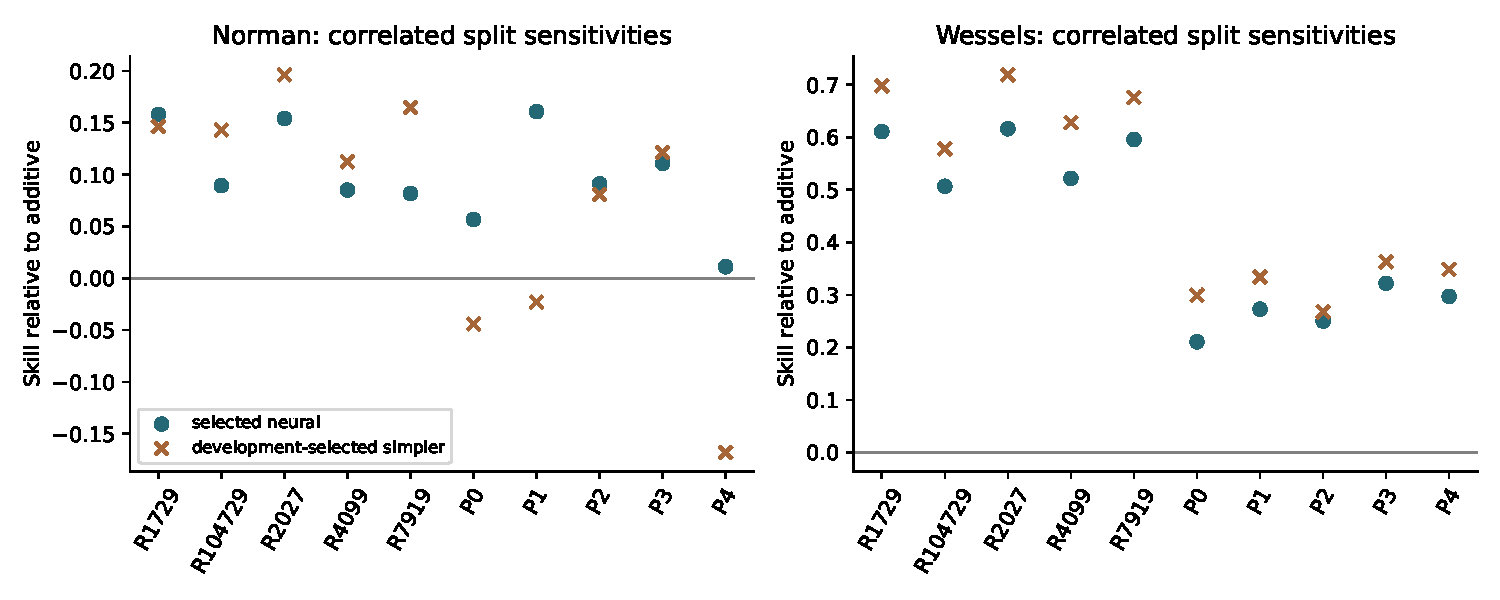
\includegraphics[width=\linewidth]{evidence/biological_robustness.pdf}\caption{Neural and simpler additive skills across registered biological splits. R denotes random-pair seeds and P partner folds.}\end{figure}}{}

\subsection{Supplementary adapted public reference}
We execute two explicitly adapted SLIM references from pinned upstream revision \texttt{5a7e9ade5d0a} \citep{slim2026}; the full identity and verified source hashes are retained in the method manifest. Its native combination fit is applied to one signed-effect pseudoprofile per condition, retaining the shared gene basis, ridge solve, mean component embedding, and separate single/double biases. We omit the native nonnegative-expression prediction clip because negative effects are valid endpoints. These changes mean the results are adapted references, not reproductions of the published expression protocol. One variant uses 64 supplied STRING dimensions and discloses external information; another substitutes PCA of the allowed observed singles, capped at 16 dimensions.

For each input variant, five development folds select from basis ranks 2, 8, and 16 and ridge penalties 0.1, 1, 10, and 100. Basis fitting uses only singles and that fold's development doubles. These supplementary comparisons were added after the primary results and do not replace the original Opal selection. On Norman, STRING and observed-single variants have MSE 0.00898725 and 0.00782653, respectively, both above the selected Opal MSE. On Wessels their MSE values are 0.00417759 and 0.00418530, both below the selected Opal value and close to the stronger internal global correction.

\IfFileExists{evidence/public_table.tex}{\begin{table}[ht]\centering\normalsize\begin{tabular}{llrr}
\toprule
Dataset & Adapted SLIM input & MSE & Additive skill \\
\midrule
Norman & STRING64 & 0.008987 & -0.055 \\
Norman & observed single PCA & 0.007827 & 0.081 \\
Wessels & STRING64 & 0.004178 & 0.700 \\
Wessels & observed single PCA & 0.004185 & 0.700 \\
\bottomrule
\end{tabular}
\caption{Late supplementary signed-effect SLIM adaptations. External STRING information and common-information observed-single PCA are reported separately.}\end{table}}{}

The original Python 3.14 environment lacks native GEARS and CPA dependencies, and CPA requires an older Python runtime. Later isolated Python 3.10 GPU runs execute both methods without changing upstream algorithm source; their aggregate-input results are reported in the context-transfer amendment. PertAdapt's supplied resources pass the retained audit, but its later full-gene float32 forward/backward feasibility probe exhausts RTX 4060 memory, and its distributed launcher requires NCCL unavailable on this Windows build. No PertAdapt biological score is reported. Environment or memory failures document execution scope, not scientific inferiority.

\subsection{Extended universe and metric controls}
An evaluator-only sensitivity uses all 33,694 original Norman genes and 20,639 Wessels genes. The learned prediction is retained on its frozen schema; outside it, the extension uses observed-single additivity, with no fitted correction. A panel selects the 20 largest absolute residual genes on one technical half and scores the opposite half, then swaps the halves. Outside-schema genes constitute 0.197\% of these Norman panel positions and none of the Wessels positions. Selected-extension MSE is 0.240990 and 0.126811, compared with additive values 0.385201 and 0.329619. This sensitivity does not show that a trained extended-universe model would recover emergent responses.

Metric controls include a zero effect, observed additivity, development mean residual, an oracle response as an explicit positive control, and 100 pair permutations of evaluator residuals. These are diagnostics rather than newly eligible candidates. On Wessels, permuted residuals retain mean response Pearson correlation 0.5638 and residual cosine 0.2516 despite MSE 0.020850, above additive MSE 0.013937. The zero-effect prediction also has positive residual cosine 0.6990 while its additive skill is negative. Positive alignment alone can therefore be driven by shared reference geometry and cannot establish useful prediction.

\subsection{Conditional technical measurement sensitivity}
Two supplementary 200-draw bootstraps resample cells within each condition and matched stratum while retaining QC, gene eligibility, normalization, fitted weights, and method predictions. Each draw uses one matched-control sample per stratum and one single sample per target, reused for every affected pair. This preserves reference sharing in the resampled profiles. It does not propagate parameter fitting, selection, biological replication, or uncertainty from predicting with newly estimated singles.

For improvement over the development-selected simpler prediction, Norman's mean difference is 0.00010518 with a technical profile percentile range $[0.00004388,0.00016553]$. Wessels' mean is $-0.00120615$ with range $[-0.00129652,-0.00113008]$. These ranges describe technical response-estimation sensitivity conditional on fixed predictions. Norman's pair-network uncertainty remains unresolved despite the positive technical range; the schemes answer different questions and must not be combined into a confirmatory confidence interval.

\subsection{Earlier chemical feasibility does not confirm transfer}

Original ComboSciPlex GSE206741 metadata records A549 cells, 24-hour exposure, and 1 micromolar per component, consistent with the primary CPA methods \citep{cpa2023}. Of 25 pair conditions, only seven have both singles in that experiment, covering six compounds. An explicitly exploratory run uses four development pairs with three-fold cross-validation and three held-out pairs, equal-well profiles, and shared plate controls. Its bounded search contains 22 configurations and omits the genetic ablation batch. Nominal embedding dimension is five.

The exploratory chemical selection is a rank-two bilinear model, with MSE $0.01222957$ and 11.44\% additive skill. A development-selected mean-residual correction has MSE $0.00994341$ and 27.99\% skill, so the bilinear selection is worse by $0.00228616$. Its additive comparison's descriptive interval crosses zero. Three held-out pairs are insufficient for confirmatory inference, model ranking, or the intended chemical method-transfer claim; these scores document source feasibility and another unfavorable structural comparison. At this historical cutoff the chemical release gate remained unresolved. The later registered EmeraldBay and D-SPIN amendments below provide larger source-qualified tasks, but do not establish positive independent transfer. Unsupported profiles cannot be reconstructed from held-out pairs.

\subsection{Coverage and independent transfer}
On a common Wessels validation population, expanded development pair coverage improves error by 16.05\% in random folds and 4.92\% in partner folds; the tested increase in single coverage changes error by about +0.03\% and -0.38\%, respectively. These are fixed-population coverage sensitivities, not evidence that pair gains scale indefinitely or that more precise matched references are unnecessary. Full menus and unfavorable architecture, annotation, state, and scale continuations remain in the supplement.

The independent D-SPIN evaluation refits the frozen EmeraldBay-selected procedure on source contexts and withholds two lineages across batches. Frozen-procedure MSE is \DspinCandidate{} versus \DspinReference{} for a source-selected pooled-pair kernel, so the superiority gate fails. A nominal 90\% source radius covers 34.3\% of held conditions. Query controls and measured singles are allowed, and the held lineages are not independently initiated cultures. This result leaves positive independent transfer and reliable shifted uncertainty unestablished.

\section{From expression composition to measured-growth prediction}
\label{sec:growth}
The experiments below are subsequent, separately registered studies. Their functional endpoint and information access differ from the historical expression benchmark. They are not revisions to its protected test scores, and growth improvements cannot be interpreted as expression improvements. Compact source-bound aggregate records accompany this section.

\subsection{First-principles restriction and the failed expression continuation}
Given measured singles $s_i,s_j$, write a combination response as $y_{ij}=s_i+s_j+\eta_{ij}$. Arbitrarily many interaction functions $\eta$ agree on the same singles. Pair supervision, additional measurements or justified structural restrictions must therefore supply the missing information. Under independent arm-estimation errors, additive-feature error and residual-target error have covariance $-\operatorname{Var}(\epsilon_i)-\operatorname{Var}(\epsilon_j)-2\operatorname{Var}(\epsilon_0)$ when each single contrast shares a control error $\epsilon_0$. Attenuating additivity may consequently correct measurement error without identifying causal antagonism.

A finite hierarchical composition test used signed same-sign and opposing-sign single-effect overlap, gene-specific slopes shrunk toward pooled coefficients, and training-fitted intercepts. Five outer and three inner folds compared it with affine calibration, reduced-rank regression and profile kernels on 88 Norman and 110 expanded Wessels fitting pairs. All these sources were already exposed development. Partner folds overlap; repeated held predictions were averaged per pair for the primary endpoint. No historical protected expression test was reopened.

\begin{table}[htbp]\centering\small
\begin{tabular}{llrr}\toprule
Source & Holdout & Composition MSE & Inner-selected reference MSE\\\midrule
Norman & Pair & 0.00621337 & 0.00608876\\
Norman & Partner & 0.00634312 & 0.00632210\\
Wessels & Pair & 0.00850956 & 0.00711547\\
Wessels & Partner & 0.00928111 & 0.00919508\\\bottomrule
\end{tabular}
\caption{The hierarchical expression-composition candidate fails all four registered comparisons. Affine calibration beats composition in every setting; the strongest reference is the Wessels kernel under random-pair holdout and affine elsewhere. These are development scores, not independent confirmation.}
\label{tab:composition-update}\end{table}

The candidate was closed rather than expanded after its loss. Its result rejects this overlap law, not the existence of biological interactions. Additional pair-response supervision motivated a separate functional task instead of a larger expression network on the same small pair banks.

\subsection{Growth data, reference and symmetric completion}
Horlbeck et al.'s double-CRISPRi screen \citep{horlbeck2018}, GEO GSE116198, supplies measured growth gamma for K562 and Jurkat. We use triple-sequencing gamma, averaging ordered guide constructs within each infection and then the two infections equally. Singles come from gene/negative-control constructs. Published genetic-interaction scores and correlations are excluded because their global construction uses pair outcomes beyond the fitting partition. The deposited gamma normalization remains a shared upstream technical dependency.

Eligibility requires at least 20 finite single observations and four finite ordered pair observations in each context and infection. The resulting bank has 81,466 canonical distinct-gene pairs and 427 supported genes in a 467-gene schema. This coverage rule does not threshold observed effect size, but missing finite phenotypes can still depend on depletion. The population is enriched for growth-related genes, not a genome-wide sample. Seed 20261021 fixes 48,879 training, 16,293 validation and 16,294 test pairs in both contexts. All guides, orientations and contexts for one pair stay together, and every query gene has training-pair support.

Let $c$ index cell context. A training-fitted reference $b_c(i,j)$ adds a ridge-calibrated correction to the observed-single sum, using its sum, absolute difference, product and optional gene-incidence terms. The completion prediction is
\begin{equation}
\widehat y_{ij,c}=b_c(i,j)+M_{ij,c},\qquad
M_c=\tfrac12(U_cV_c^{\mathsf T}+V_cU_c^{\mathsf T}).
\end{equation}
Unlike a positive-semidefinite factorization, this symmetric indefinite matrix permits positive and negative residual structure. A sharing candidate replaces $M_c$ by a common symmetric matrix plus context-private factors. Independent, pooled-only and common/private alternatives have equal factor parameter budgets within each registered rank comparison. The joint rank-$r$ model uses shared rank $r$ and private rank $r/2$; independent models use rank $r$ per context, and pooled-only uses rank $2r$.

Training-only scales and coefficients are fitted before validation selects references, ranks 8/16, penalties 0.001/0.01 and checkpoints every 25 steps. Adam uses learning rate 0.03, one fixed initialization and a 500-step cap. Baselines include zero, original-single sum and minimum, scalar calibration, calibrated gene main effects, independent completion and pooled-only completion. No test outcome participates in selection. The joint model must improve at least 2\% over the validation-selected strongest non-joint reference in both contexts with below-zero upper conditional loss-difference bounds; test-best alternatives are not retrospectively promoted.

\begin{table}[htbp]\centering\small
\begin{tabular}{lrrr}\toprule
Context & Main-effect MSE & Independent MSE & Joint MSE\\\midrule
K562 & 0.00187049 & 0.00137593 & 0.00136626\\
Jurkat & 0.00050049 & 0.00042630 & 0.00045576\\\bottomrule
\end{tabular}
\caption{Locked within-source growth test. Independent completion improves over calibrated main effects by 26.44\% and 14.82\%. Joint sharing gains only 0.70\% in K562 and loses 6.91\% in Jurkat against the stronger completion reference, failing promotion. MSE units are growth gamma squared and cannot be pooled with expression MSE.}
\label{tab:growth-internal}\end{table}

Validation retains independent rank 8, penalty 0.01, step 300 for K562 and rank 16, penalty 0.01, step 200 for Jurkat. The joint winner uses rank 8, penalty 0.01, step 125. The finite fit took 18.72 seconds and about 916 MiB peak working set on one numerical thread. Independent completion is a specialized within-source predictor; the common/private hypothesis is failed relative to that strong reference, not a newly competitive architecture.

\subsection{Frozen external reference-growth evaluation}
The retained K562 predictor was frozen before scoring reference growth in the environmental screen of Herken et al. \citep{herken2026}, GSE312636, and the PARPi screen of Simpson et al. \citep{simpson2023}, GSE284018. Environmental experiments 1/2 and PARPi 2022/2023 remain four cohorts from two studies, each retaining two infection replicates. They share laboratory lineage and cannot count as four independent laboratories or studies. Three sequencing runs in PARPi 2022 are technical reads merged before analysis.

Only untreated/DMSO gamma is compared with the frozen predictor. Drug response, sensitization and globally fitted interaction scores are different endpoints. Whole-library filtering requires each guide's mean of infection-specific median T0 counts to exceed 35 in both positions and each construct to exceed 50 in both T0 samples. Add ten to surviving counts, form log2 endpoint/T0 enrichment, subtract the double-negative-control median per infection and divide by author-supplied reference population doublings. Sequencing-fraction normalization cancels after this centering. The environmental authors use endpoint-based guide coverage; our registered T0-only harmonization deliberately differs to avoid excluding strong observed depletion. It is not exact published-score reproduction. Environmental experiment 2 has 2,023 incomplete constructs, excluded rather than zero-imputed; missingness may nevertheless be response-dependent.

Canonical pair targets average at least two distinct ordered guide constructs within each infection, then weight infections equally. Guide orientations are subsamples, not biological replicates. The primary panel contains supported-gene pairs absent from the entire original eligible bank, with at least 50 pairs and ten genes per cohort. This is \emph{bank-novel}, not necessarily never measured. Original test, validation and training overlaps remain separate as previously scored, selection-exposed and repeatability strata.

The model and same-information references retain original singles and coefficients. No external single replaces an input, and no intercept, scale, factor or checkpoint is fitted to external outcomes. MSE against mean infection targets is primary; infection-specific errors, bias, MAE and Pearson correlation are retained. Two thousand conditional pair and gene-resampling draws use seed 20261020. Gene resampling weights each edge by the product of resampled endpoint multiplicities. These intervals describe sensitivity conditional on measured panels and cultures, not population-level uncertainty from two infections. Promotion requires at least 2\% mean-target MSE gain over frozen main effects in every qualifying cohort, improvement in each infection, below-zero upper gene-resampling bounds and no loss to the other fixed simple references.

\begin{table}[htbp]\centering\small
\begin{tabular}{lrrrr}\toprule
Cohort & Pairs / genes & Completion & Main effects & Original minimum\\\midrule
Environmental 1 & 130 / 17 & 0.0710602 & 0.0695619 & 0.0358322\\
Environmental 2 & 130 / 17 & 0.0504016 & 0.0493793 & 0.0255072\\
PARPi 2022 & 423 / 30 & 0.1060987 & 0.1048554 & 0.0670913\\
PARPi 2023 & 411 / 30 & 0.1067118 & 0.1055719 & 0.0672618\\\bottomrule
\end{tabular}
\caption{Frozen K562 external bank-novel MSE. All panels qualify and all fail promotion. Completion MSE is 2.15\%, 2.07\%, 1.19\% and 1.08\% higher than frozen main effects. The panels overlap; their summed rows are not independent pair samples.}
\label{tab:growth-external}\end{table}

Completion-minus-main-effect gene-resampling bounds are $[-0.002278,0.005191]$, $[-0.001911,0.004077]$, $[-0.001419,0.003735]$ and $[-0.001494,0.003670]$. All include zero, so this is failed superiority, not established general harm from completion. Original-single minimum is substantially better in every cohort, and zero also beats completion on the two PARPi bank-novel panels. Original-test overlap shows no consistent completion gain either. The original within-source results are preserved; no failed source-transfer claim is rescued by post-result tuning.

\subsection{What the graph and assay audits change}
The four bank-novel panels comprise only 509 unique pairs. Environmental panels are identical sets of 130; PARPi 2023's 411 are a subset of 2022's 423. Environmental overlap with PARPi is 44 or 38 pairs. All 509 occur in the original raw Horlbeck table, but fail the joint-context finite-coverage rule. Some exclusions from K562 evaluation arise solely from Jurkat coverage. Thus ``bank-novel'' describes training eligibility, not the absence of original biological measurement.

These panels are nearly complete subgraphs among 17 or 30 genes, while their endpoint genes have low original eligible degree, median 285 versus 426 over all active genes. The external test therefore combines source shift with a graph-support shift. A no-fit audit on the exposed original test uses training-degree tertiles fixed before subgroup losses: 8,270 pairs touching the lowest tertile still show gains of 21.08\% in K562 and 14.40\% in Jurkat; the 112 lowest/lowest pairs show 14.07\% and 14.40\%. This weakens a sole explanation based on low degree, but does not simulate an entirely missing gene block. Only four original test pairs have both endpoints in the 37-gene union of external bank-novel genes, too few for the registered descriptive-interval minimum. Neither subgroup replay nor the external result identifies a causal graph-support contribution.

Original/external single-effect Pearson correlations are 0.161, 0.308, $-0.030$ and $-0.038$, with large mean changes. A positive scalar rescaling alone cannot repair those centered correlations. External measured-single minimum MSE is 0.00584, 0.00915, 0.00253 and 0.00234 on the same primary panels. This is extra information, not a fair same-input score for adapted Opal. Opposite-infection single-to-pair checks and count-threshold sensitivities retain their exploratory role. Reagent choice, perturbation strength, duration, cell state, depletion floors, normalization and informative missingness remain confounded.

A later no-fit diagnostic adds a measured source-cohort residual for the \emph{same} pair to target-cohort minimum singles. For 130 environmental and 411 PARPi matched pairs, residual correlations are 0.722 and 0.845; the fixed transfer improves minimum-single MSE in both directions. Cross-study overlaps contain only 38 or 44 pairs and have wider conditional bounds. All twelve directed point estimates improve on minimum, but four bounds include zero. This does not predict an unseen combination: its source input includes that combination's measured response. Edge shuffling also destroys gene-associated structure, so aligned/shuffled differences cannot uniquely identify pair-specific biology. Reused exposed outcomes, overlapping panels and this additional label access prohibit a new confirmatory or model-promotion claim.

\subsection{Local-reference replacement does not transport the old correction}
A separate frozen no-fit diagnostic gives the predictor external minimum singles, while retaining exactly the old completion correction $\widehat y^{\rm old}_{ij}-b^{\rm old}(i,j)$ with unit weight. Minimum is computed within infection before infection averaging; no source pair outcome supplies the correction, and no external coefficient or checkpoint is selected. This is an exposed successor diagnostic with extra information, not a revision to the equal-input external test.

\begin{table}[htbp]\centering\small
\begin{tabular}{lrrr}\toprule
Cohort & Local minimum & Minimum + old correction & Gain (\%)\\\midrule
Environmental 1 & 0.00583726 & 0.00580404 & 0.57\\
Environmental 2 & 0.00914504 & 0.00871926 & 4.66\\
PARPi 2022 & 0.00252622 & 0.00313029 & $-23.91$\\
PARPi 2023 & 0.00234228 & 0.00294654 & $-25.80$\\\bottomrule
\end{tabular}
\caption{Exploratory reference replacement at fixed correction weight one. Environmental conditional paired gene-resampling bounds include zero; both PARPi loss-difference intervals are entirely positive. No correction-weight rescue is fitted.}
\label{tab:growth-reference-swap}\end{table}

The PARPi loss-difference bounds are $[0.000225,0.001051]$ and $[0.000265,0.001011]$, conditional on these cultures and genes. Losses persist in both opposite-infection directions. Adding the correction to local additive singles also raises primary MSE in all four cohorts. Thus better local main effects alone do not make the historical correction transportable at unit weight. The correction/reference decomposition is dependent on its source calibration; the result rejects this direct transplant, not all assay adaptation or the existence of interactions.

\subsection{Cross-infection held-pair development retains a limited signal}
An explicitly exploratory continuation reuses the original pair split to ask whether residual alignment predicts the opposite deposited infection. Source-infection singles and training pairs fit fixed-alpha references; source-infection validation selects the reference and checkpoint. Opposite-infection pair outcomes enter only final scoring. One rank-8 independent completion uses penalty 0.01, 500 steps and seed 20261022. A matched negative control applies one fixed shared permutation to training residual pair labels, preserving cross-context residual covariance while breaking pair alignment. Ten reference fits and four completion fits take 9.77 seconds; no rank, penalty or seed search occurs.

\begin{table}[htbp]\centering\small
\begin{tabular}{llrrrr}\toprule
Context & Infection & Selected node & Aligned & Shuffled & Gain (\%)\\\midrule
K562 & $1\to2$ & 0.00452043 & 0.00433089 & 0.00485093 & 4.19\\
Jurkat & $1\to2$ & 0.00171504 & 0.00165254 & 0.00173088 & 3.64\\
K562 & $2\to1$ & 0.00573598 & 0.00526993 & 0.00591978 & 8.12\\
Jurkat & $2\to1$ & 0.00174425 & 0.00168909 & 0.00176404 & 3.16\\\bottomrule
\end{tabular}
\caption{Exposed-source held-pair cross-infection MSE. Reference selection uses source validation only; the same canonical test pairs occur in both directions. Gains pass the registered development gate relative to selected node effects, but are not four independent confirmations or consistent superiority to every simple reference.}
\label{tab:growth-infections}\end{table}

Two thousand positive gene-node multiplier draws assign independent Exp(1) weights to genes and endpoint-product weights to edges, unlike the discrete gene resampling in the external test. All four aligned-minus-node upper bounds are below zero, and every aligned fit beats its shuffled control. These are conditional dyadic sensitivity bounds with no formal biological-population coverage guarantee. Importantly, the calibrated-single reference on Jurkat $1\to2$ has MSE 0.00164975, slightly better than aligned completion's 0.00165254. This post-scoring comparator disclosure is not used to refit a replacement, but prevents claiming universal simple-baseline superiority.

After separately fitted node references, residual infection correlations are 0.384 in K562 and 0.240 in Jurkat, versus raw response correlations 0.879 and 0.938. Raw-growth repeatability is therefore not evidence that interaction residuals are equally reliable. The aligned gains support useful within-study pair-associated structure after this reference adjustment; shared guides, common processing and incomplete main-effect calibration remain alternative explanations. A passed exploratory gate permits an untouched-source experiment, not architecture promotion or reversal of the external failure.

\subsection{Scientific decision and exposure boundary}
The expression-overlap and cross-context-sharing hypotheses are closed, and unchanged-model external superiority is failed. Independent completion remains a source-conditional reference. The later infection experiment is promising only as exposed development relative to its source-selected node baseline; the stronger calibrated comparison qualifies that result. None of these studies demonstrates transferable mechanisms, unseen-gene prediction, improved expression from growth training, calibrated biological uncertainty or frontier performance.

The next falsifiable improvement concerns jointly validated assay-local reference and residual prediction with graph-matched support, not an indiscriminate architecture expansion. The fixed reference-replacement result rules out assuming that the old residual can simply be added to better local singles. Development should first test incremental pair prediction above minimum, additive and calibrated-single/main-effect references, with a negative control and an explicit missing-block task when that is the intended use. A subsequent compatible source must remain outside selection. Original test sets, all four external cohorts and the repeated diagnostic panels are already exposed; repartitioning or a newly frozen comparison cannot make them untouched. The present revision reports existing evidence and performs no biological fitting.


Metadata-only follow-up identifies SPIDR \citep{fielden2025} as a possible future source, not an executed accuracy result. Its library shares 41 supported genes and 820 distinct supported pairs, 136 absent from the original eligible bank, before observed coverage is known. The broad screen is RPE-1 TP53-knockout T14/T0 log-fold change, with deliberate guide mismatches and cultures split after transduction. It is not interchangeable with K562 per-doubling gamma. Response Table 8 was not opened in this qualification. Any use requires a separately registered context/endpoint task and an outcome-independent guide/coverage rule; library overlap does not certify usable response supervision.



\section{Six-task assay-local growth delivery}
\label{sec:v1-delivery}
The later frozen tournament and October 27 delivery use six already exposed tasks: Horlbeck K562 and Jurkat, two environmental reference cohorts, and PARPi 2022 and 2023. This is source-local supervised development, not a new external confirmation of the earlier predictor. Each procedure receives 16,000 TRAIN and 4,000 VALIDATION canonical pair labels, source-local measured singles and the same support population as its registered comparators. Five disjoint within-gene-fold missing-block test populations are pooled per task. Every query gene has at least two distinct training partners. These block populations differ from the original random-pair growth split above and must not be combined as one benchmark.

The finite menu includes sixteen fixed simple references, validation-selected simple, kernel and neural families, signed completion and three residual-label shuffle policies. Selection uses registered validation data. The full ledger retains infection-target errors, coverage, MAE, bias, correlation and conditional gene sensitivities. Gene resampling describes sensitivity on this graph, rather than uncertainty over independent studies.

Historical rank 8 denotes factor width in $M=(UV^{\mathsf T}+VU^{\mathsf T})/2$. Its algebraic rank is at most 16, with at most eight positive and eight negative directions. It is neither a verified rank-eight matrix nor an eight-dimensional biological interaction space. Delivery stores the selected symmetric operator losslessly; compression changes storage, not predictions.

\begin{table}[htbp]\centering\small
\begin{tabular}{lrrrr}\toprule
Task & Test pairs & Simple MSE & Completion MSE & Gain\\\midrule
K562 & 16,210 & 0.00190091929 & 0.00179069074 & 5.80\%\\
Jurkat & 16,210 & 0.000507630148 & 0.000486775245 & 4.11\%\\
Environmental 1 & 9,833 & 0.000551581712 & 0.000412898098 & 25.14\%\\
Environmental 2 & 9,833 & 0.000727352832 & 0.000518265563 & 28.75\%\\
PARPi 2022 & 29,016 & 0.000308097243 & 0.000254004302 & 17.56\%\\
PARPi 2023 & 28,651 & 0.000302940513 & 0.000260679297 & 13.95\%\\
\bottomrule\end{tabular}
\caption{Six-task assay-local development, pooled over five disjoint test blocks. Coverage is 100\% on each registered population. Gains compare the selected policy to validation-selected simple references. Jurkat fails the unchanged 5\% all-task criterion. Scores are not measurements of a single exported fold-0 checkpoint.}
\label{tab:v1-growth}\end{table}


Completion leads this finite kernel/neural menu and beats every registered fixed simple reference and shuffle policy on the pooled populations. Nevertheless, the unchanged all-task rule requires at least 5\% improvement in every task. Jurkat reaches only 4.11\%, so the program fails and no model is scientifically promoted. No test-based rescue or general method ranking follows.

The usable delivery fixes fold 0 in advance for every task and copies each original validation-selected checkpoint. The pooled five-fold scores in Table~\ref{tab:v1-growth} characterize the training procedure, not a single exported checkpoint or an all-data refit. A separately recorded training reproduction matched all 168 saved states and prediction vectors. Release preparation replayed 17,176 saved queries exactly across six checkpoints without fitting, computing a new score or opening test targets. Engineering replay establishes computational identity in its recorded environment, not biological replication.

\subsection{Negative experiments that constrain interpretation}
The local block study reports gains against selected simple references, but its fixed native NAIAD comparator has lower MSE than completion on PARPi 2022 only. Small family-selector gains in two tasks do not establish an optimized public-method ranking. Exact guide/arm matching and nonlinear-single controls leave local completion advantages without identifying molecular interactions or excluding all technical pair effects.

Neither tested pair-label budget is nominated. The 5,000-label policy passes no task, and the 20,000-label policy misses the required gain in original K562 and Jurkat despite full query coverage. The later finite tournament's Jurkat failure is separate evidence under its own comparator menu and split contract.

The strongest nonlinear-single nuisance comparison stopped before completion fitting or test scoring because stored predictions failed legacy replay. Numerical audits localized batch-dependent whitening arithmetic and tested alternate reductions, precision and layouts. A versioned fixed-order predictor passes registered caller-invariance controls but differs from the historical predictor by $4.660858310412408\times10^{-8}$, above the unchanged $10^{-12}$ tolerance. Determinism does not settle the strongest-reference scientific question, which remains unanswered.

Historical state/context, dose and model-series studies retain unfavorable outcomes. Learned state models fail matched simple-reference gates; dose interpolation is restricted to known compounds and states while extrapolation fails; global chemical-pair development finds no pair-kernel improvement. These results and source-qualification refusals remain in the archived manuscript and original evidence. They are not converted into new independent tests.

\section{Discussion and limitations}
Opal's usable claim is assay-local prediction under explicit measured-single and pair-label access. A symmetric correction can capture broad calibration, source-specific structure or technical pair effects as well as biological interactions. Predictive gains cannot distinguish these explanations. Growth and expression endpoints differ and cannot validate one another.

Frozen cross-study growth transfer fails, while later local fitting succeeds on several exposed tasks. The latter uses different information and does not reverse the former. The external bank-novel panels contain 509 unique pairs present in the original raw table but excluded from the eligible bank, confounding assay shift with support-block shift. Same-pair residual transfer supplies a measured source outcome for the queried pair; it is a different task from unseen-pair completion.

Population means hide cell heterogeneity, source-specific coverage rules restrict the gene/pair universe, and selection/refitting uncertainty is not fully propagated. Technical halves, guide orientations, shared controls, infection readings and dependent folds are not independently initiated biological replicates. Conditional resampling and ensemble spread are not calibrated biological intervals. Support-based abstention is not a calibrated probability of prediction failure.

This release establishes no biological discovery, causal understanding, reliable independent-study generalization, frontier-level superiority or clinically validated prediction. Negative experiments and failed criteria delimit the claim. Source hashes and replay support auditability without certifying source authenticity, legal clearance or biological independence.

\section*{Data and code availability}
Opal v1.0.0 source is maintained at \url{https://github.com/TheTinyIntelLab/opal}. GitHub contains MIT-licensed original code, tests, manuscript sources and PDF, compact aggregate evidence, protocols, provenance and notices. Raw datasets, trained checkpoints, full reference/prediction banks, private correspondence and local plans are excluded. Models will have a separate Hugging Face release. No public model URL, archive DOI or arXiv identifier is claimed here.

Growth sources are GSE116198 \citep{horlbeck2018}, GSE312636 \citep{herken2026} and the pinned official PARPi repository associated with GSE284018 \citep{simpson2023}. Source-specific terms remain separate from Opal's MIT code. The Horlbeck author deposit declares CC BY 4.0, but exact equivalence with the acquired GEO mirror remains unverified. Environmental article/software licensing is not treated as blanket relicensing of GEO counts. The PARPi repository explicitly covers code and data with CC BY 4.0. Historical redistribution caveats remain documented for the separate model delivery.

The original update is bound to \texttt{paper/evidence/model\_development\_20261020.json}; the six-task delivery is bound to \texttt{results/model-delivery-20261027/benchmark.json} and its unchanged original ledger. Table~\ref{tab:v1-growth} and the v1 claim snapshot are generated from that benchmark. Original registrations, selections and scores are preserved. The complete pre-v1 manuscript and long supplement are archived under \texttt{paper/historical/v0.1.3-pre-v1/}, with input manifests and retained evidence dependencies. No biological training ran during release preparation.

A public checkout supports code tests and aggregate replay, but every biological result cannot be reproduced without separately obtained local assets. Release validation is recorded in \texttt{results/release-v1.0.0/validation.json}; historical test counts apply to their identified revisions.

\section*{Ethics and author declarations}
The work reuses published perturbation data and reports computational analyses, with no new human recruitment, animal work or prospective intervention study. Source publications describe original oversight. No new ethics approval or clinical validation is claimed.

Arjun Vijay Prakash is the sole author, an independent high school student at City Montessori School, and maintains The Tiny Intelligence Lab as an independent research project. The work received no funding and the author declares no competing interests.

\section*{AI assistance disclosure}
OpenAI Codex assisted with implementation, experimental orchestration and manuscript editing. Numerical claims refer to retained artifacts. AI assistance does not establish authorship, independent replication or expert validation; the author is responsible for the final code, interpretation, attribution and text.

\clearpage
\begingroup\small
\bibliographystyle{plainnat}
\bibliography{references}
\endgroup
\end{document}
